\chapter{How a Key Opens a Lock}
This chapter presents the basic workings of pin tumbler locks, and the vocabulary used in the rest of this booklet.
The terms used to describe locks and lock parts vary from manufacture to manufacture and from city to city, so even if you already understand the basic workings of locks, you should look at figure 2.1 for the vocabulary.

Knowing how a lock works when it is opened by a key is only part of what you need to know.
You also need to know how a lock responds to picking. Chapters 3 and 5 present models which will help you understand a lock's response to picking.

Figure 2.1 introduces the vocabulary of real locks.
The key is inserted into the \textit{keyway} of the \textit{plug}.
The protrusions on the side of the \textit{keyway} are called \textit{wards}.
Wards restrict the set of keys that can be inserted into the plug.
The plug is a cylinder which can rotate when the proper key is fully inserted.
The non-rotating part of the lock is called the \textit{hull}.
The first pin touched by the key is called pin one.
The remaining pins are numbered increasingly toward the rear of the lock.

The proper key lifts each pin pair until the gap between the \textit{key pin} and the \textit{driver pin} reaches the \textit{sheer line}.
When all the pins are in this position, the plug can rotate and the lock can be opened.
An incorrect key will leave some of the pins protruding between the hull and the plug, and these pins will prevent the plug from rotating.

\begin{figure}
    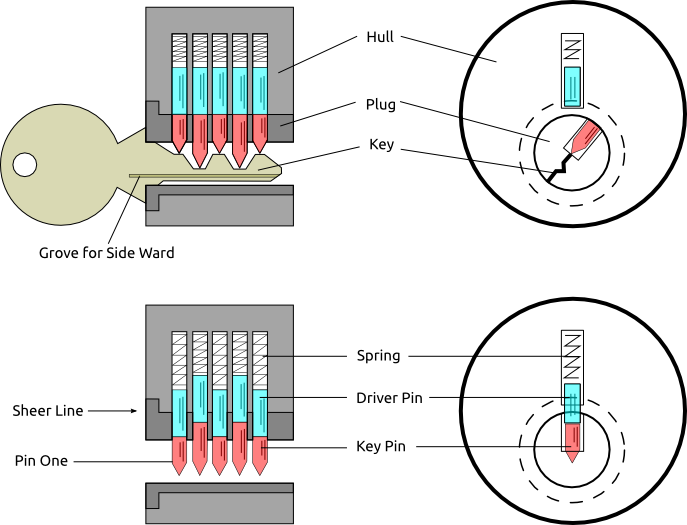
\includegraphics[width=\textwidth]{figure2.1}
    \caption{Workings of pin tumbler locks}
\end{figure}
